\documentclass{beamer}
\usepackage[utf8]{inputenc}
\usepackage{float}

\usetheme{Madrid}
\usecolortheme{default}

%Information to be included in the title page:
\title[Geodesica en Espacio de Minkowski] %optional
{Geodesica Alrededor de una Particula con Masa en el Espacio de Minkowski}

\author[] % (optional, for multiple authors)
{Manuel Angel Garcia\inst{1} \and Carlos Andres Llanos\inst{1}}

\institute[] % (optional)
{
  \inst{1}%
  Facultad de Fisica\\
  Universidad Nacional de Colombia
}

\date[2023] % (optional)
{Clase de Metodos Geometricos}

\logo{
\includegraphics[height=1cm]{Logo-unal}}

\begin{document}

\frame{\titlepage}

\begin{frame}
\frametitle{Metrica de Schwarzschild}

Partiendo de la metrica de Minkowski en esfericas: 
\begin{gather*}
  ds^2 _{\text{Minkowski }}  = - dt^2 + dr^2 + r^2 d \Omega^2
\end{gather*}

Necesitamos una metrical que mantenga la forma del angulo solido, así que podemos multiplicarlo por una funcion radial:
\begin{gather*}
  ds^2 = - e ^ {2 \alpha (r) } dt^2 + e ^ {2 \beta(r) } dr^2 + e ^ {2\gamma(r)}r^2 d \Omega^2 
\end{gather*}

Aplicamos la siguiente transformacion: 
\begin{gather*}
  \bar r = e ^ {\gamma(r)}r \qquad \qquad d\bar r = \left(1 + r \frac{d \gamma  }{d r }\right)e ^ {\gamma } dr 
\end{gather*}
La metrica nos queda: 
\begin{gather*}
  ds^2 = - e ^ {2 \alpha(r)}dt^2 + \left(1 + r \frac{d \gamma  }{d r }\right)^ {-2 } e ^ {2 \beta (r) - 2 \gamma (r) }d \bar r ^2 + \bar r ^2 d \Omega^2 
\end{gather*}

\end{frame}


%%%%%%%%%%%%%%%%%%%%%%%%%%%%%%%%%%%%%%%%%%


\begin{frame}
\frametitle{Metrica de Schwarzschild}

\begin{gather*}
  ds^2 = - e ^ {2 \alpha(r)}dt^2 + \left(1 + r \frac{d \gamma  }{d r }\right)^ {-2 } e ^ {2 \beta (r) - 2 \gamma (r) }d \bar r ^2 + \bar r ^2 d \Omega^2 
\end{gather*}
Haciendo $ \bar r \rightarrow r  $ obtenemos que: $ \left(1 + r \frac{d \gamma  }{d r }\right)^ {-2 } e ^ {2 \beta (r) - 2 \gamma (r) } \rightarrow e ^ {2 \beta } $

\hfill 

\hfill 

Por lo tanto podemos escribir la metrica como: 

\begin{gather*}
  ds^2 = - e ^ {2\alpha(r)}dt^2 + e ^ {2 \beta (r) } dr^2 + r^2 d \Omega^2  
\end{gather*}

\end{frame}


%%%%%%%%%%%%%%%%%%%%%%%%%%%%%%%%%%%%%%%%%%


\begin{frame}
\frametitle{Metrica de Schwarzschild}

\begin{gather*}
  ds^2 = - e ^ {2\alpha(r)}dt^2 + e ^ {2 \beta (r) } dr^2 + r^2 d \Omega^2  
\end{gather*}
Calculamos los simbolos de Christoffel:
\begin{align*}
  &\Gamma_{t r}^t=\partial _r \alpha \qquad &&\Gamma_{t t}^r=e^{2(\alpha-\beta)} \partial_r \alpha \qquad &&&\Gamma_{r r}^{r}=\partial_r \beta \\
  &\Gamma_{r \theta}^\theta=\frac{1}{r} \qquad &&\Gamma_{\theta \theta}^r=-r e^{-2 \beta} \qquad &&&\Gamma_{r \phi}^\phi=\frac{1}{r} \\
  &\Gamma_{\phi \phi}^r=-r e^{-2 \beta} \sin ^2 \theta \qquad &&\Gamma_{\phi \phi}^\theta=-\sin \theta \cos \theta \qquad &&&\Gamma_{\theta \phi}^\phi=\frac{\cos \theta}{\sin \theta}
\end{align*}
\end{frame}


%%%%%%%%%%%%%%%%%%%%%%%%%%%%%%%%%%%%%%%%%%


\begin{frame}
\frametitle{Metrica de Schwarzschild}

Con los simbolos de Christoffel podemos obtener el tensor de Riemann: 

\begin{align*}
  &R_{r t r}^{t}=\partial_r \alpha \partial_r \beta-\partial_r^2 \alpha-(\partial_r \alpha)^2 \\
  &R_{\theta t \theta }^{t}=-r e^{-2 \beta} \partial_r \alpha \\
  &R_{\phi t \phi}^t=-r e^{-2 \beta} \sin ^2 \theta \partial_r \alpha \\
  &R_{\theta r \theta}^r=r e^{-2 \beta} \partial_r \beta \\
  &R_{\phi r \phi}^{r}=r e^{-2 \beta} \sin ^2 \theta \partial_r \beta \\
  &R _{\phi \theta \phi } ^ {\theta }=\left(1-e^{-2 \beta}\right) \sin ^2 \theta 
\end{align*}


\end{frame}


%%%%%%%%%%%%%%%%%%%%%%%%%%%%%%%%%%%%%%%%%%


\begin{frame}
\frametitle{Metrica de Schwarzschild}

Tomando la contraccion obtenemos el tensor de Ricci: 

\begin{align*}
  &R_{t t}=e^{2(\alpha-\theta)}\left[\partial_r^2 \alpha+\left(\partial_r \alpha\right)^2-\partial_r \alpha \partial_r \beta+\frac{2}{r} \partial_r \alpha\right] \\
  &R_{r r}=-\partial_r^2 \alpha-\left(\partial_r \alpha\right)^2+\partial_r \alpha \partial_r \beta+\frac{2}{r} \partial_r \beta \\
  &R_{\theta \theta}=e^{-2 \beta}\left[r\left(\partial_r \beta-\partial_r \alpha\right)-1\right]+1 \\
  &R_{\phi \phi}=\sin ^2 \theta \ \ R_{\theta \phi}
\end{align*}


\end{frame}


%%%%%%%%%%%%%%%%%%%%%%%%%%%%%%%%%%%%%%%%%%


\begin{frame}
\frametitle{Metrica de Schwarzschild}
Reemplazamos el tensor de Ricci en la ecuacion de campo de Einstein en el vacio para hallar $ \alpha  $ y $ \beta  $: 
\begin{gather*}
  R _{\mu \nu }  - \frac{1}{2} R g _{\mu \nu }  = 0  
\end{gather*}
Obteniendo: 
\begin{align*}
  e ^ {2 (\beta - \alpha )} e ^ {2 (\alpha - \beta )} &\left[\partial_r^2 \alpha + (\partial_r \alpha )^2 - \partial_r \alpha \partial_r \beta + \frac{2 }{r } \partial_r \alpha \right] \\ 
  &- \partial_r^2 \alpha - (\partial_r \alpha)^2 + \partial_r \alpha \partial_r \beta + \frac{2}{r} \partial_r \beta = 0 \\ 
  \Longrightarrow \frac{2 }{r } \partial_r \alpha + \frac{2 }{r } \partial_r \beta = 0 
\end{align*}
Para que se cumpla esta ecuacion necesitamos que $ \alpha = - \beta + c  $
\end{frame}


%%%%%%%%%%%%%%%%%%%%%%%%%%%%%%%%%%%%%%%%%%


\begin{frame}
\frametitle{Metrica de Schwarzschild}
\begin{gather*}
  \alpha = - \beta  
\end{gather*}
Reemplazando en $ R _{\theta \theta }  = 0  $: 
\begin{gather*}
  e ^ {2\alpha }(2r \partial_r \alpha + 1 ) = 1 \Longrightarrow \partial_r (r e ^ {2\alpha }) = 1 
\end{gather*}
Resolviendo esta ecuacion obtenemos: 
\begin{gather*}
  e ^ {2\alpha } = 1 - \frac{R_s }{r } 
\end{gather*}
De esta forma obtenemos que podemos escribir la metrica como: 
\begin{gather*}
  ds^2 = - \left(1 - \frac{R_s }{r }\right)dt^2 + \left(1 - \frac{R_s }{r}\right) ^ {-1 } dr^2 + r^2 d \Omega^2  
\end{gather*}
\end{frame}


%%%%%%%%%%%%%%%%%%%%%%%%%%%%%%%%%%%%%%%%%%


\begin{frame}
\frametitle{Metrica de Schwarzschild}
EXPLICAR POR QUÉ EL RADIO DE Schwarzschild ES $R_S=2GM$
\end{frame}


%%%%%%%%%%%%%%%%%%%%%%%%%%%%%%%%%%%%%%%%%%


\begin{frame}
\frametitle{Geodesicas de Schwarzschild}
\begin{gather*}
  ds^2 = - \left(1 - \frac{2GM }{r }\right)dt^2 + \left(1 - \frac{2GM }{r}\right) ^ {-1 } dr^2 + r^2 d \Omega^2  
\end{gather*}

Calculamos los simbolos de Christoffel
\begin{figure}[H]
  \begin{center}
    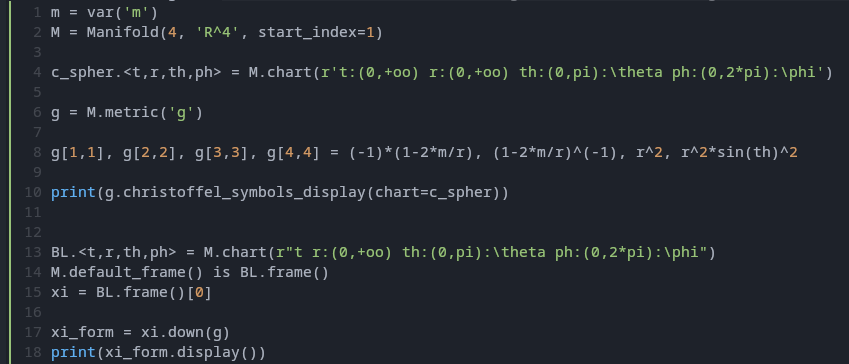
\includegraphics[width=0.95\textwidth]{sage.png}
  \end{center}
\end{figure}
\end{frame}


%%%%%%%%%%%%%%%%%%%%%%%%%%%%%%%%%%%%%%%%%%


\begin{frame}
\frametitle{Geodesicas de Schwarzschild}
Simbolo de Christoffel para la metrica: 
\begin{gather*}
\begin{array}{lcl} \Gamma_{ \phantom{\, t} \, t \, r }^{ \, t \phantom{\, t} \phantom{\, r} } & = & -\frac{M}{2 \, M r - r^{2}} \\ \Gamma_{ \phantom{\, r} \, t \, t }^{ \, r \phantom{\, t} \phantom{\, t} } & = & -\frac{2 \, M^{2} - M r}{r^{3}} \\ \Gamma_{ \phantom{\, r} \, r \, r }^{ \, r \phantom{\, r} \phantom{\, r} } & = & \frac{M}{2 \, M r - r^{2}} \\ \Gamma_{ \phantom{\, r} \, {\theta} \, {\theta} }^{ \, r \phantom{\, {\theta}} \phantom{\, {\theta}} } & = & 2 \, M - r \\ \Gamma_{ \phantom{\, r} \, {\phi} \, {\phi} }^{ \, r \phantom{\, {\phi}} \phantom{\, {\phi}} } & = & {\left(2 \, M - r\right)} \sin\left({\theta}\right)^{2} \\ \Gamma_{ \phantom{\, {\theta}} \, r \, {\theta} }^{ \, {\theta} \phantom{\, r} \phantom{\, {\theta}} } & = & \frac{1}{r} \\ \Gamma_{ \phantom{\, {\theta}} \, {\phi} \, {\phi} }^{ \, {\theta} \phantom{\, {\phi}} \phantom{\, {\phi}} } & = & -\cos\left({\theta}\right) \sin\left({\theta}\right) \\ \Gamma_{ \phantom{\, {\phi}} \, r \, {\phi} }^{ \, {\phi} \phantom{\, r} \phantom{\, {\phi}} } & = & \frac{1}{r} \\ \Gamma_{ \phantom{\, {\phi}} \, {\theta} \, {\phi} }^{ \, {\phi} \phantom{\, {\theta}} \phantom{\, {\phi}} } & = & \frac{\cos\left({\theta}\right)}{\sin\left({\theta}\right)} \end{array}
\end{gather*}
\end{frame}

%%%%%%%%%%%%%%%%%%%%%%%%%%%%%%%%%%%%%%%%%%


\begin{frame}
\frametitle{Geodesicas de Schwarzschild}

Reemplazando los simbolos de Christoffel en la ecuacion de la geodesica: 
\begin{gather*}
  \ddot t + \frac{2M}{r(r-2M)}\dot r \dot t = 0\\
  \ddot r + \frac{M}{r^3}(r-2M)\dot t^2 - \frac{M\dot r}{r(r-2M)}-(r-2M)\dot \phi^2=0 \\
  \ddot \phi + \frac{2}{r} \dot \phi \dot r = 0 
\end{gather*}
\end{frame}

\end{document}
